\newcommand{\C}{\mathcal{C}\xspace}
\subsection{Price of Fairness}
\label{sec:comparison}

The efficient fairness/accuracy frontiers pictured in Figure
\ref{fig:pareto} can be compared across data sets in a qualitative
sense --- e.g. to see that in some datasets, the fairness penalty can
be substantially decreased with little cost to accuracy. However, they
are difficult to compare quantitatively, because the scale of the
fairness loss differs substantially from data set to data set. In this
section, we give a cross-dataset comparison using a measure (which we
call {\em Price of Fairness\/}) which has the effect of normalizing
the fairness loss across data sets to lie on the same scale.

For a given data set and regression type (linear or logistic), let
$\vw^*$ be the optimal model absent any fairness penalty (i.e. the
empirical risk minimizer when the fairness ``regularization'' weight
$\lambda = 0$). This model will suffer some fairness penalty: it
represents the ``maximally unfair'' point on the fairness/accuracy
frontiers from Figure \ref{fig:pareto}. For each dataset, we will fix
a normalization such that this fairness penalty is rescaled to be 1,
and ask for the cost (in terms of the relative increase in mean
squared error) of constraining our predictor to have fairness penalty
$\alpha \leq 1$. Equivalently, this is measuring the relative increase
in $\mse$ that results from constraining a predictor to have fairness
penalty that is no more than \emph{an $\alpha$ fraction of the
  fairness penalty of the unconstrained optimal predictor}.

More formally, let $\vw^* = \arg\min_{\vw} \ell_\cP(\vw)$.
For any value of $\alpha\in[0,1]$ we define the \emph{price of fairness}
(\pof) as follows:
\[
\text{\pof}(\alpha) = \frac{\min_{\vw} \ell_\cP(\vw) \text{ subject to }   f_\cP(\vw) \leq \alpha  f_\cP(\vw^*) }{\ell_\cP(\vw^*)}.
\]

Note that by definition, $\pof(\alpha) \geq 1$, $\pof(1) = 1$, and that $\pof(\alpha)$ increases monotonically as $\alpha$ decreases. Larger values represent more severe costs for imposing fairness constraints that ask that the measure of unfairness be small relative to the unconstrained optimum. It is important to note that because this measure asks for the cost of \emph{relative} improvements over the unconstrained optimum, it can be, for example, that the PoF for one fairness penalty case is larger than for another, even if the \emph{absolute} fairness loss for both the numerator and the denominator is smaller in the second case. With this observation in mind, we can move to the empirical findings.

Figure~\ref{fig:pof} displays the PoF on each of the $6$ datasets we study, for each fairness regularizer (individual, hybrid, and group), and for the single and separate model case. We first note that even when normalized on a common scale, we continue to see the diversity across datasets that was apparent in Figure~\ref{fig:pareto}. For some datasets (e.g. COMPAS and Sentencing), increasing the fairness constraint by decreasing $\alpha$ has only a mild cost in terms of error. For others (e.g. Communities and Crime, and Law School), the cost increases steadily as we decrease $\alpha$. 

Next, we observe that with this normalization, although the difference between separate and single models remains small on most datasets, on two datasets, differences emerge. In the Law School dataset, restricting to a single model leads to a significantly higher PoF when considering the group fairness metric, compared to allowing separate models. In contrast, on the Adult dataset, restricting to a single model substantially \emph{reduces} the PoF when considering the individual fairness metric. 

Finally, this normalization allows us to observe variation across fairness penalties in the \emph{rate of change} in the PoF as $\alpha$ is decreased. In some datasets (e.g. Communities and Crime, and Sentencing), the PoF changes in lock-step across all measures of unfairness. However, for others (e.g. Default), the PoF increases substantially with $\alpha$ when we consider group or hybrid fairness measures, but is much more stable for individual fairness. 

\begin{figure}[h!]
\begin{minipage}[b]{0.32\textwidth}
\centering
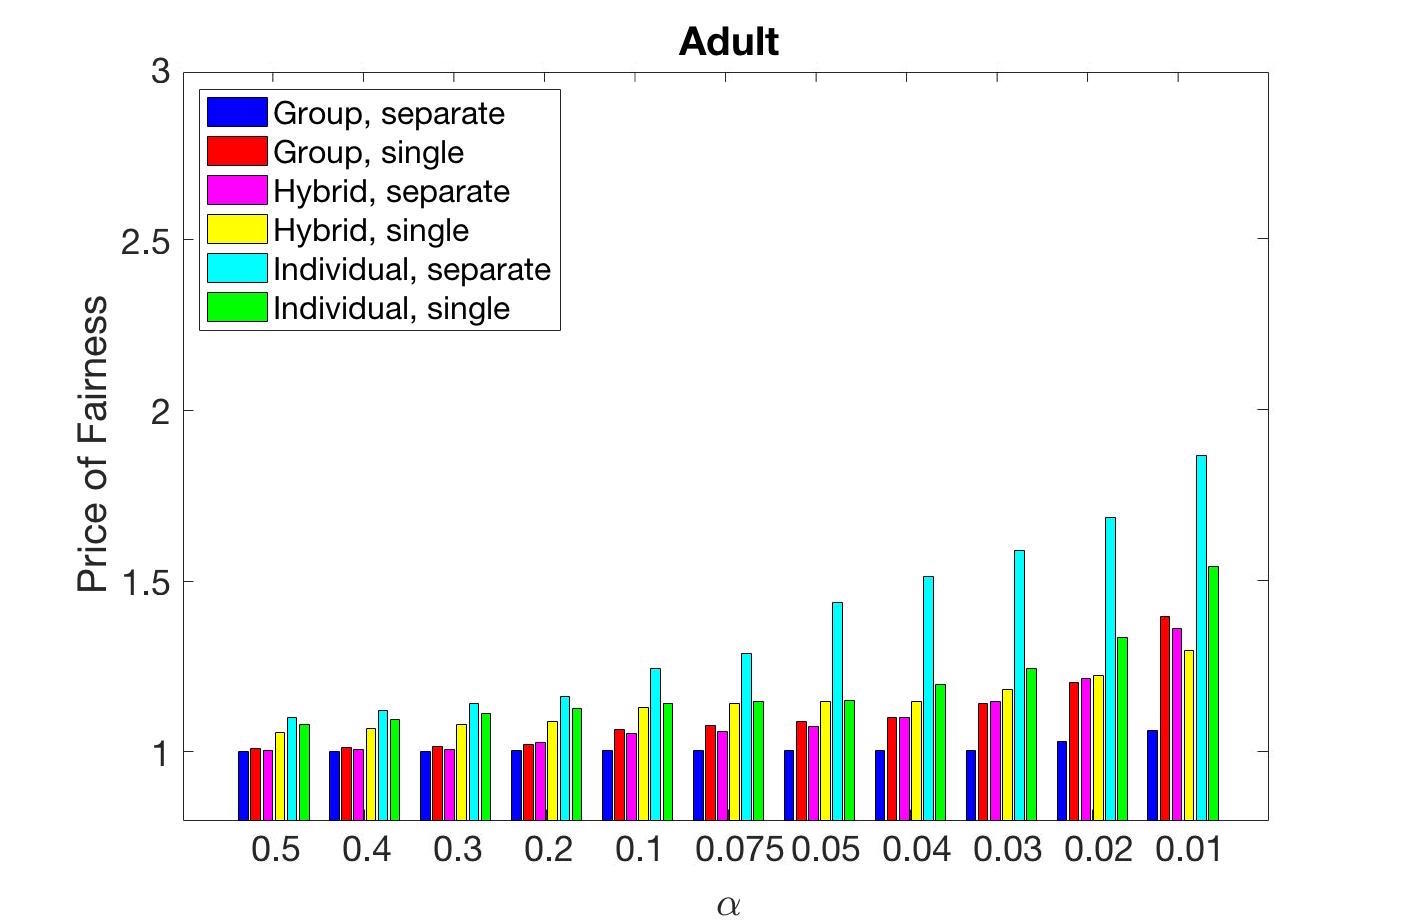
\includegraphics[width=5.8cm]{./figures/pof-twoversusone-adult.jpg}
%\caption{}
\end{minipage}
\begin{minipage}[b]{0.32\textwidth}
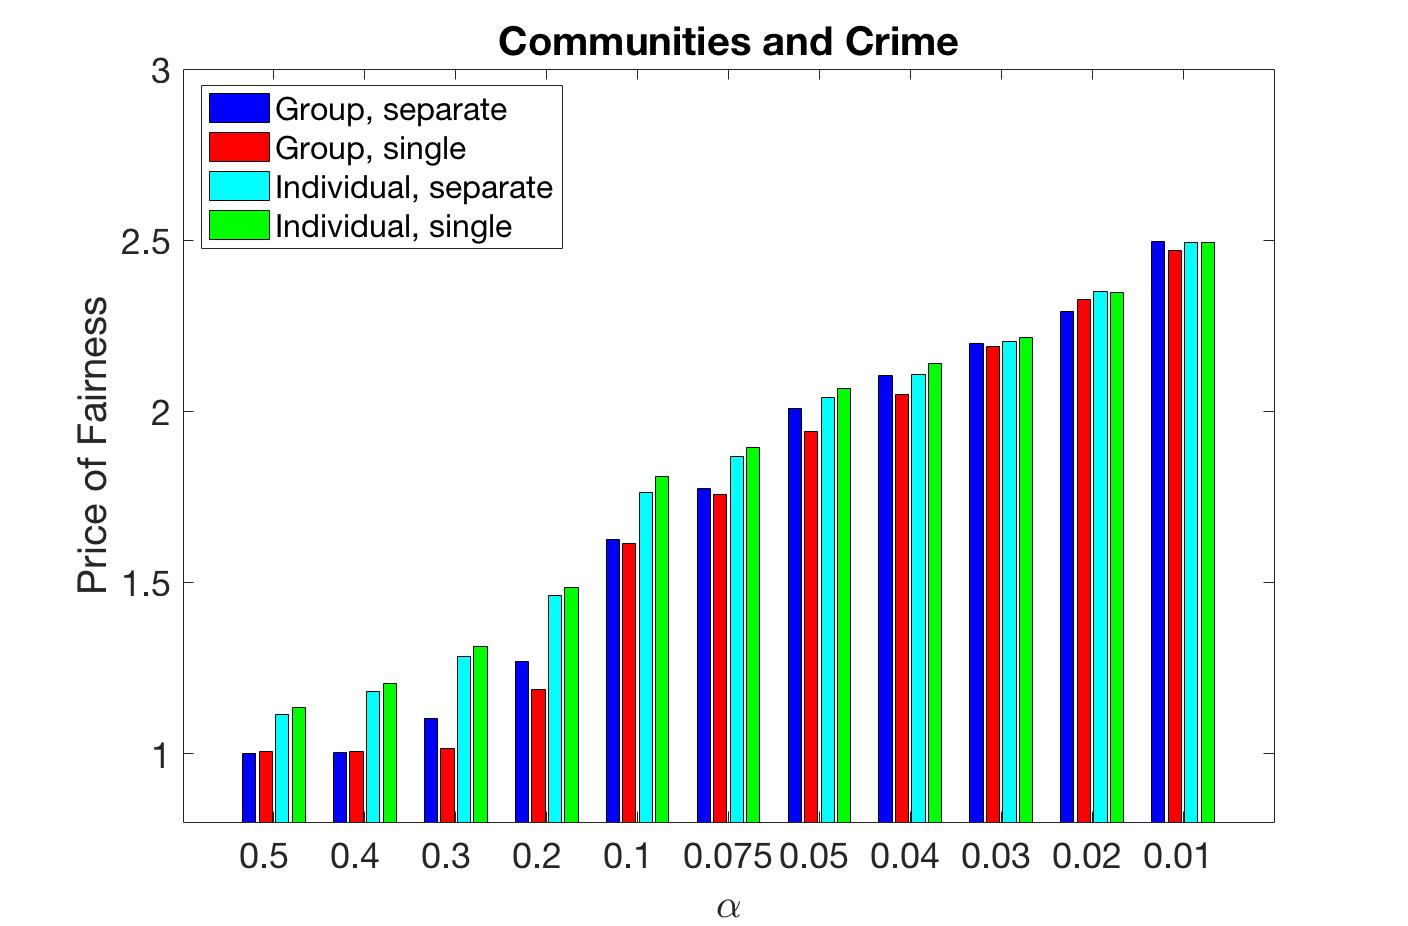
\includegraphics[width=5.8cm]{./figures/pof-twoversusone-communities.jpg}
%\caption{}
\end{minipage}
\begin{minipage}[b]{0.32\textwidth}
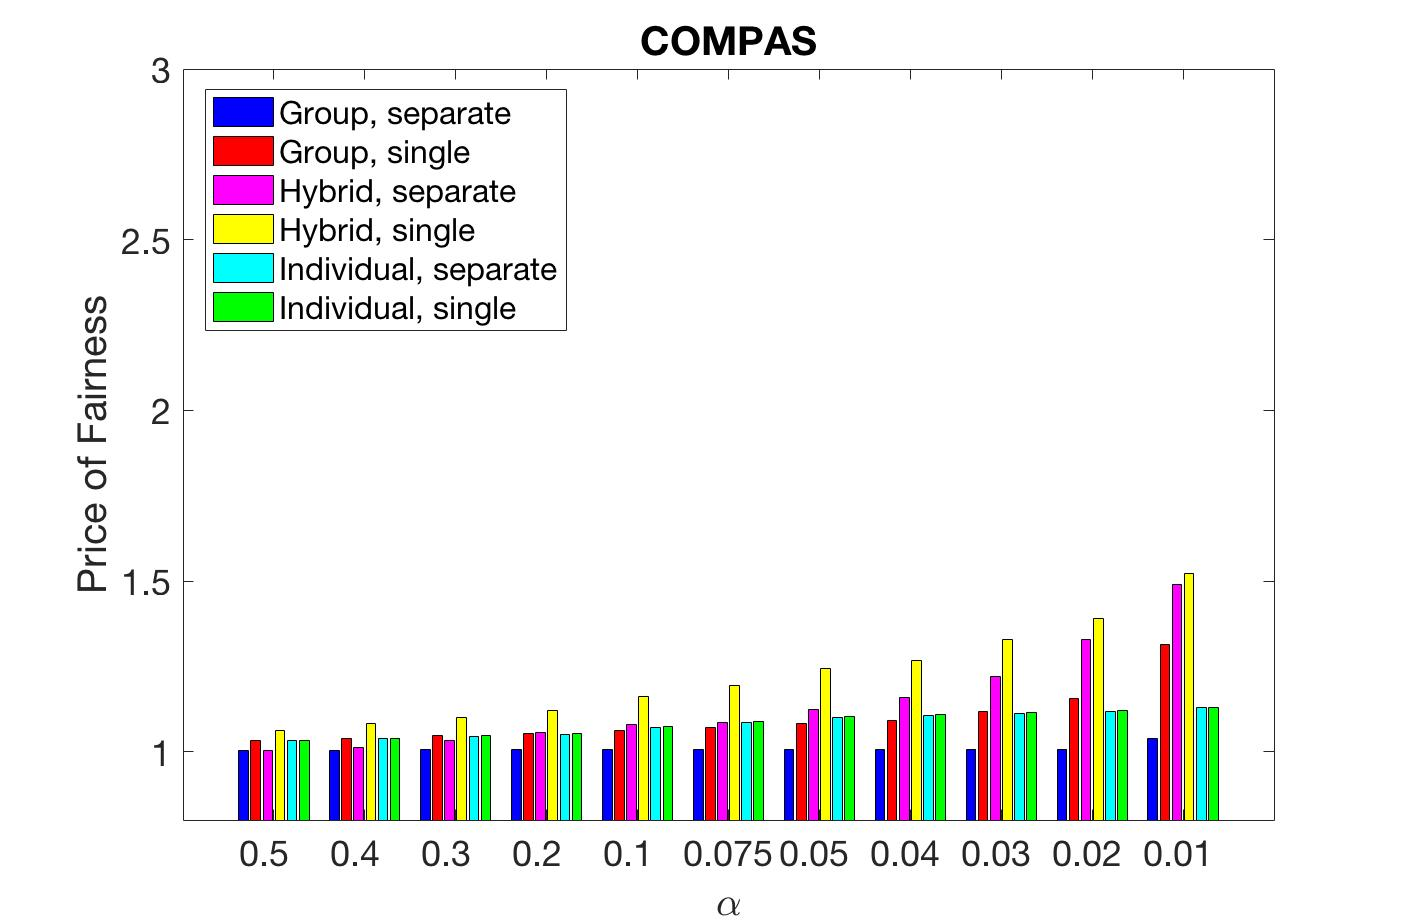
\includegraphics[width=5.8cm]{./figures/pof-twoversusone-compas.jpg}
%\caption{}
\end{minipage}\\
\begin{minipage}[b]{0.32\textwidth}
\centering
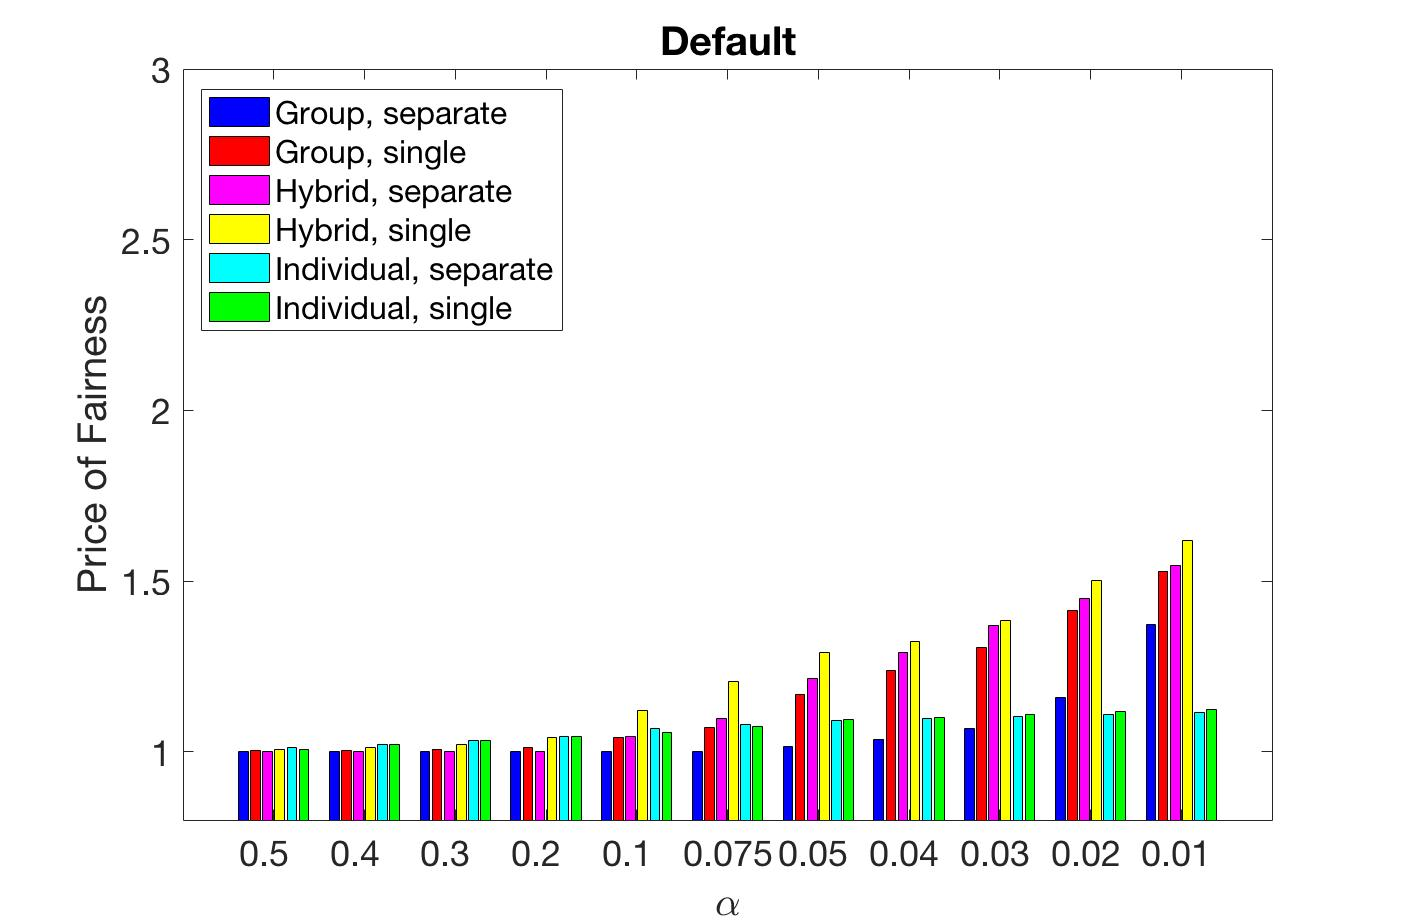
\includegraphics[width=5.8cm]{./figures/pof-twoversusone-default.jpg}
%\caption{}
\end{minipage}
\begin{minipage}[b]{0.32\textwidth}
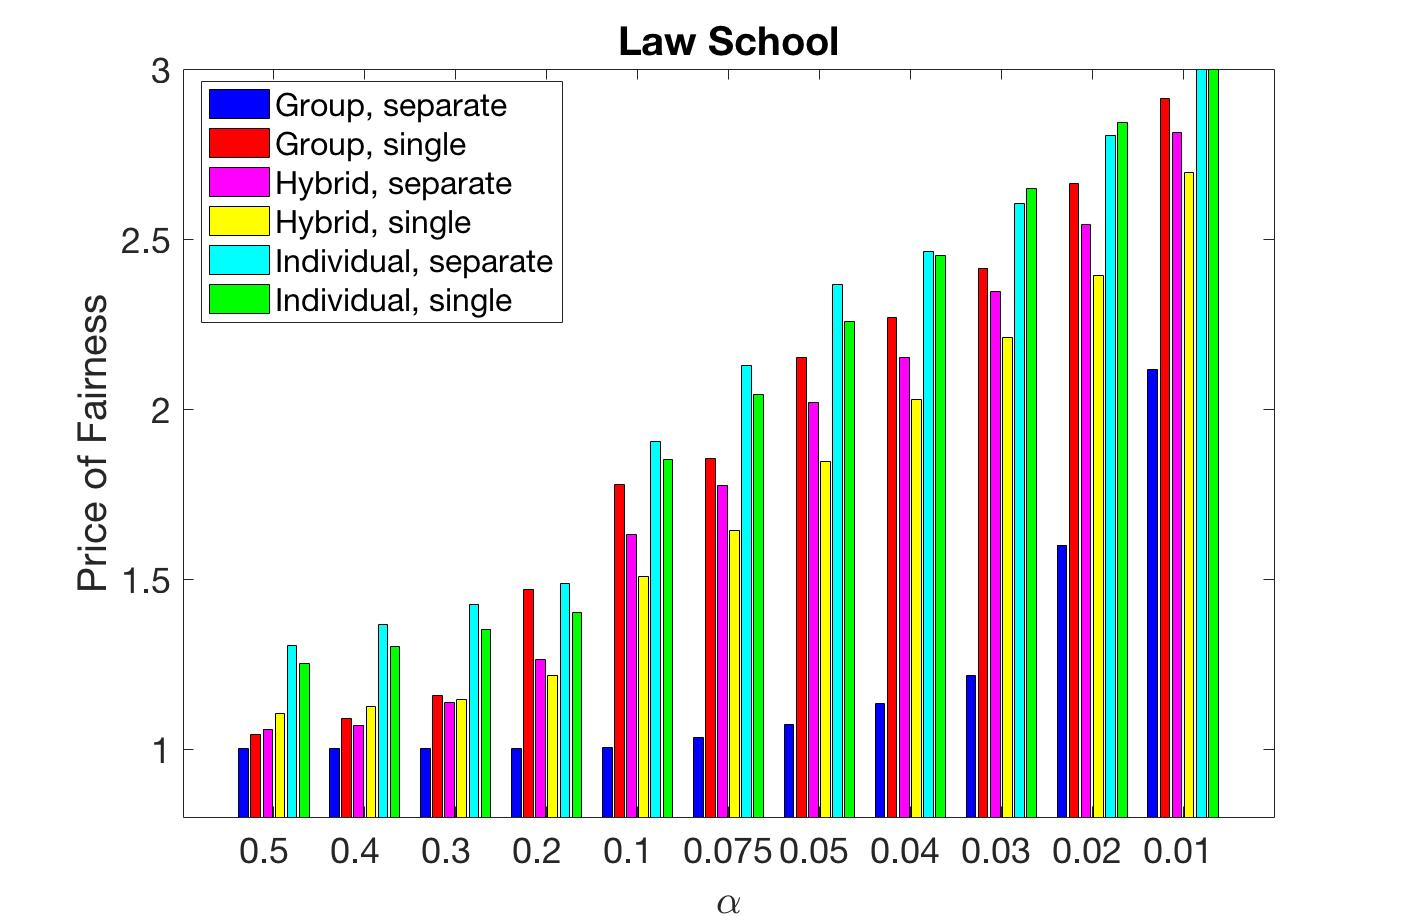
\includegraphics[width=5.8cm]{./figures/pof-twoversusone-law.jpg}
%\caption{}
\end{minipage}
\begin{minipage}[b]{0.32\textwidth}
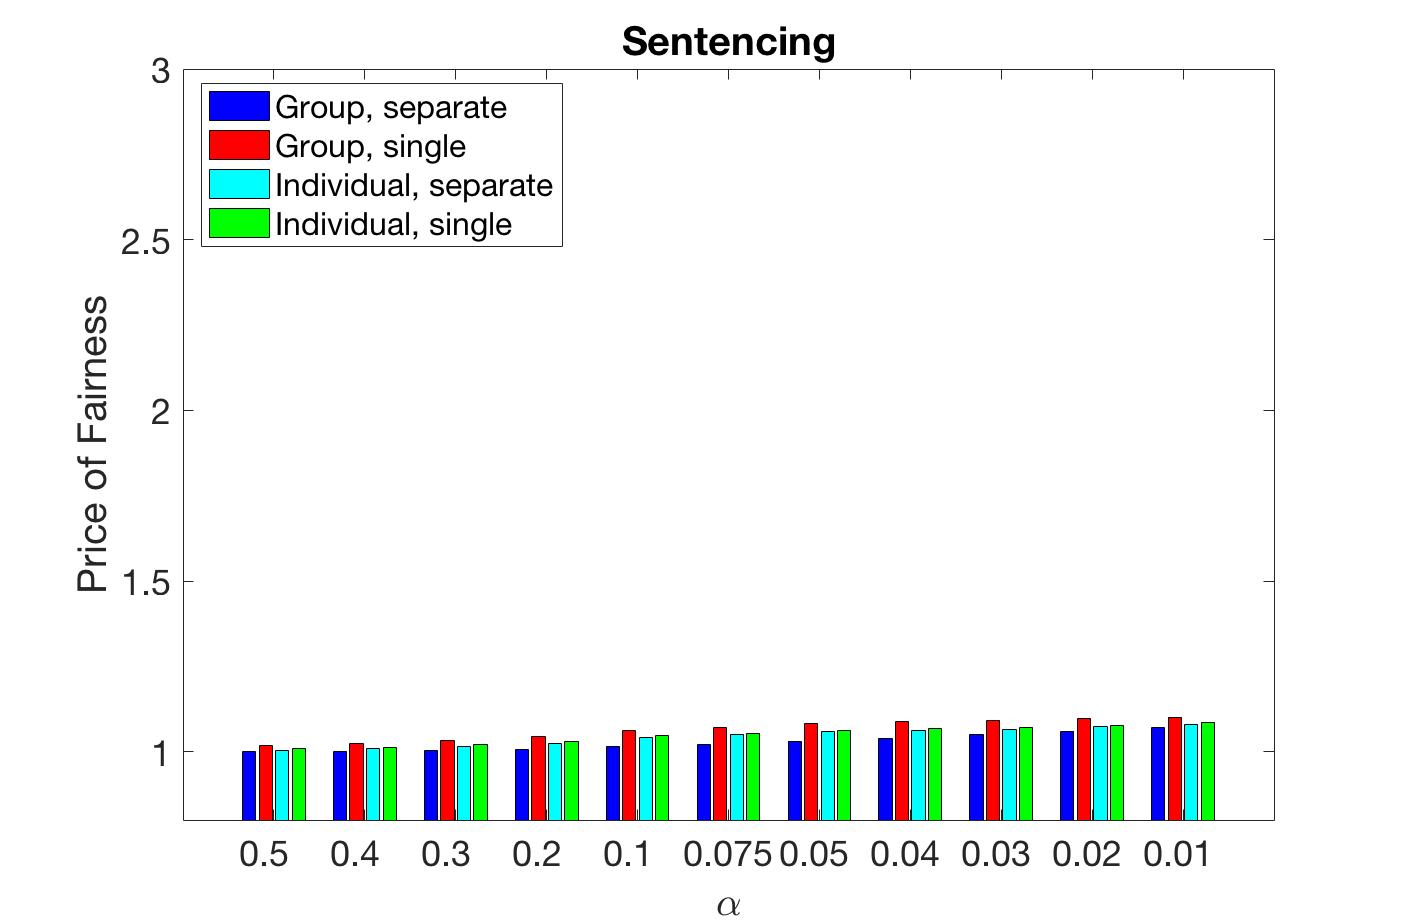
\includegraphics[width=5.8cm]{./figures/pof-twoversusone-philadelphia.jpg}
%\caption{}
\end{minipage}
\caption{The ``Price of Fairness'' across data sets, for each type of fairness regularizer, in both the single and separate model case.}   \label{fig:pof}
\end{figure} 
